\documentclass[conference]{IEEEtran}
% Add the compsoc option for Computer Society conferences.
%
% If IEEEtran.cls has not been installed into the LaTeX system files,
% manually specify the path to it like:
% \documentclass[conference]{../sty/IEEEtran}


% *** CITATION PACKAGES ***
%
\usepackage{cite}

% *** GRAPHICS RELATED PACKAGES ***
%
\usepackage[pdftex]{graphicx}
% declare the path(s) where your graphic files are
\graphicspath{{./images/}}
% and their extensions so you won't have to specify these with
% every instance of \includegraphics
\DeclareGraphicsExtensions{.png}

% *** MATH PACKAGES ***
%
\usepackage[cmex10]{amsmath}

% *** SPECIALIZED LIST PACKAGES ***
% *** SUBFIGURE PACKAGES ***
\usepackage[tight,footnotesize]{subfigure}

% *** PDF, URL AND HYPERLINK PACKAGES ***
%
\usepackage{url}

% correct bad hyphenation here
\hyphenation{op-tical net-works semi-conduc-tor}


\begin{document}
%
% paper title
% can use linebreaks \\ within to get better formatting as desired
\title{Lifelong Learning: A case study of punting balls}


% author names and affiliations
% use a multiple column layout for up to three different
% affiliations
\author{\IEEEauthorblockN{Ravikiran Janardhana}
\IEEEauthorblockA{Department of Computer Science\\
University of North Carolina at Chapel Hill\\
Email: ravikirn@cs.unc.edu}}

% conference papers do not typically use \thanks and this command
% is locked out in conference mode. If really needed, such as for
% the acknowledgment of grants, issue a \IEEEoverridecommandlockouts
% after \documentclass

% for over three affiliations, or if they all won't fit within the width
% of the page, use this alternative format:
% 

% make the title area
\maketitle

\begin{abstract}
%\boldmath
Designing robots that learn by themselves to perform complex real-world tasks is a still-open challenge for the field of Robotics and Artificial Intelligence. In this project, I use the case study of punting balls as a lifelong learning problem. The robot is fed with demonstrations of punting a variety of balls and records the target distanced acheived and updates the physics model of the punt with each demonstration. The learning process is continuous and not stagnant and as a result of this, the internal model needs to be bounded by a finite memory and we need to represent model/data in an efficient format. After the initial demonstrations, the robot is able to predict the launch velocity and the angle of elevation given any new ball and a target distance to reach. The efficient data representation of the model is achieved using the combination of Gaussian Mixture Models (GMM) and Gaussian Mixture Regression (GMR) and I show that the memory required to store the such an internal model compared to storing each of the individual demonstrations is substantially small. Using this physics model, the robot can predict the configuration to punt a new ball to reach a target distance with high accuracy.
\end{abstract}

\section{Introduction}
Throughout the last decades, the field of robotics has produced a large variety of approaches to automate and perform a variety of tasks. Despite significant progress in virtually all aspects of robotics science, most of today's robots are specialized to perform a narrow set of tasks in a very particular kind of environment. Most robots employ specialized controllers that have been carefully designed by hand, using extensive knowledge of the robot, its environment and its task. If one is interested in building autonomous multi-purpose robots, such approaches face some serious bottlenecks such as knowledge bottleneck (not aware of all the dynamics at design time), engineering bottleneck (most models are explictly hand coded) and tractability bottleneck (high computational complexity). 

Machine learning aims to overcome these limitations, by enabling a robot to collect its knowledge on-the-fly, through realworld experimentation. If a robot is placed in a novel, unknown environment, or faced with a novel tak for which no a priori solution is known, a robot that learns can collect new experiences, acquire new skills, and eventually perform new tasks all by itself. For example, in \cite{ref:1} a robot manipulator is described which learns to insert a peg in a hole without prior knowledge regarding the manipulator or the hole. Maes and Brooks \cite{ref:2} successfully applied learning techniques to coordinating leg motion for an insect-like robot. Their approach, too, operates in the absence of a model of the dynamics of the system. Learning techniques have frequently come to bear in situations where the physical world is extremely hard to model by hand (e.g., the characteristics of noisy sensors). For example, Pomerleau describes a computer system that learns to steer a vehicle driving at 55mph on public highways, based on input sensor data from a video camera \cite{ref:3}. Learning techniques have also successfully been applied to speed-up robot control, by observing the statistical regularities of "typical" situations (like typical robot and environment configurations), and compiling more compact controllers for the frequently encountered. For example, Mitchell \cite{ref:4} describes an approach in which a mobile robot becomes increasingly reactive, by using observations to compile fast rules out of a database of domain knowledge. 

However, there is a principle shortcoming in most of to date's rigorous learning approaches. Most of the robot control learning approaches focus on learning to achieve single, isolated performance tasks. If one is interested in learning with a minimum amount of initial knowledge, as is often the case in approaches to robot learning, such approaches have a critical limiting factor the number of training examples required for successful generalization. The more complex the task at hand and the lesser is known about the problem beforehand, the more training data is necessary to achieve the task. In many robotics domains the collection of training data is an expensive undertaking due to the slowness of robotics hardware. Hence, it does not surprise that the time required for real-world experimentation has frequently been found to be the limiting factor that prevents rigorous machine learning techniques from being truly successful in robotics. 

The task of learning from scratch can be significantly simplified by considering robots that face whole collections of control learning problems over their entire lifetime. In such a lifelong robot learning scenario \cite{ref:5, ref:6}, learning tasks are related in that they all play in the same environment, and that they involve the the same robot hardware. Lifelong learning scenarios open the opportunity for the transfer of knowledge across tasks. Complex tasks, which might require huge amounts of training data when faced in isolation, can conceivably be achieved much faster if a robot manages to exploit previously learned knowledge. For example, a lifelong learning robot might acquire general-purpose knowledge about itself and its environment, or acquire generally useful skills that can be applied in the context of multiple tasks. Such functions, once learned, can be applied to speed up learning in new tasks. 

In order to transfer knowledge across various tasks, first we need to have an efficient physical model representation of any task at hand rather than storing each of the individual demonstration as is. Also, it is expected that the robot continues to learn via new demonstrations and this places a limit on the amount of data it can store. In this project, I have used the example of punting a ball and analyzed the physical model required to replicate the punt trajectories. I present a novel method to store the punt physical model extracted using Gaussian Mixture Models (GMM) in an efficient matrix structure which can be later used to retrieve trajectories using Gaussian Mixture Regresstion given any new configuration. By doing so, I show that the memory required to store the model using my method is substantially smaller when compared to storing all of the trajectory data. I also show that the retrieved trajectory from this model is highly accurate without losing too much of information.

\section{Method}
\subsection{Physics model of a punt}
Equations for hang time and horizontal distance can be derived from the projectile equations of motion
\begin{equation}
y(t) = v_{y}t - \frac{1}{2}a_{y}t^{2}
\end{equation}
\begin{equation}
x(t) = v_{x}t
\end{equation}
where y and x are the height and horizontal displacements respectively, $v_{y}$ and $v_{x}$ are its vertical and horizontal velocities, $a_{y}$ is its vertical acceleration, and t is its time in flight. An expression for hang time, T, results from solving Eqn 1 for t when y = 0 and a = 9.8m/$s^{2}$ ,
\begin{equation}
T = \frac{2v_{0} sin(\theta_{0})}{9.8}
\end{equation}
where $v_{0}$ and $\theta_{0}$ are initial velocity and launch angle respectively. 

However, the above equations neglect air resistance which can lead to a substantial error when dealing in a practical environment. Air resistance, or drag, is a viscous force in a direction opposing the velocity of the projectile. Air drag, W, is given by the relation,
\begin{equation}
W = \frac{1}{2}\rho{C_{D}}Av^{2} 
\end{equation}
where $\rho$ is the air density, $C_{D}$ is the drag coefficient, A is the cross-sectional area of the projectile normal to the trajectory and v is the speed of the projectile relative to the air.

In order to include the drag into the physics model, the acceleration in x and y directions have to be suitably modified as below,
\begin{equation}
a_{x} = -C_{D}vv_{x}
\end{equation}
\begin{equation}
a_{y} = -C_{D}vv_{y} - g
\end{equation}
where g = 9.8m/$s^{2}$ and the negative sign indicates that these forces are acting against the launch velocity. 

% Table 1
\begin{table}[t]
\centering
\caption{Variation of Model parameters}
\begin{tabular}{  | c | c | c | c | c |}
  \hline
  Model & $v_{0}$ & $\theta_{0}$ & $max_{x}$ & $t_{total}$\\
  \hline 
  Without Drag  & 31.3 m/s  & 45$^{\circ}$ & 100.01 m & 4.52 secs  \\ 
  \hline
  With Drag  & 31.3 m/s  & 45$^{\circ}$ & 63.21 m & 3.6 secs  \\
  \hline
  With Drag Corrected  & 43.31 m/s  & 44$^{\circ}$ & 100.01 m & 4.7 secs  \\
  \hline
\end{tabular}
\label{tab:tab1}
\end{table}

%% Figure1
\begin{figure}[!t]
\centering
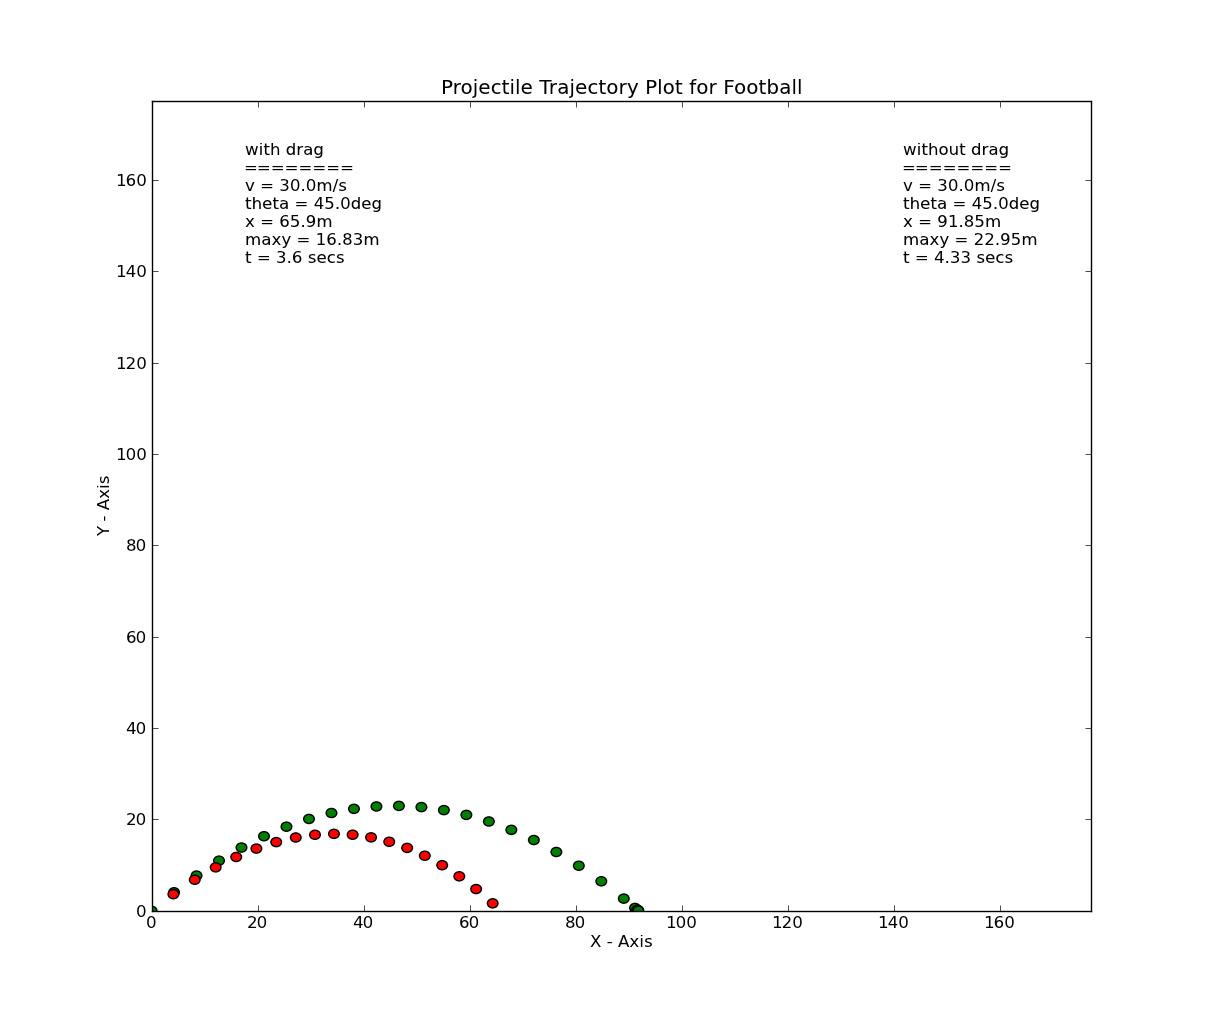
\includegraphics[width=3.5in]{fig1}
\caption{Projectile with and without drag}
\label{fig:fig1}
\end{figure}

Consider a scenario where the robot needs to predict the launch velocity and angle so that a football reaches a target distance of 100 meters assuming the Drag Coefficient $C_{D}$ in air is 0.006.  Table ~\ref{tab:tab1} shows the variation of maximum horizontal distance ($max_{x}$) and total time taken ($t_{total}$) by the projectile with and without taking drag forces into account. Using the learned model, the robot now predicts the correct launch velocity and angle to reach the target distance using a greedy optimizer. Figure ~\ref{fig:fig1} shows the pictorial representation of the scenario described by Table ~\ref{tab:tab1}.  

By varying the drag coefficient $C_{D}$, we can introduce noise in the trajectory distribution and obtain various trajectories which we can use for training the robot. Figure ~\ref{fig:fig2} shows different noisy trajectories obtained for different values of $C_{D}$.

%% Figure2
\begin{figure}[!t]
\centering
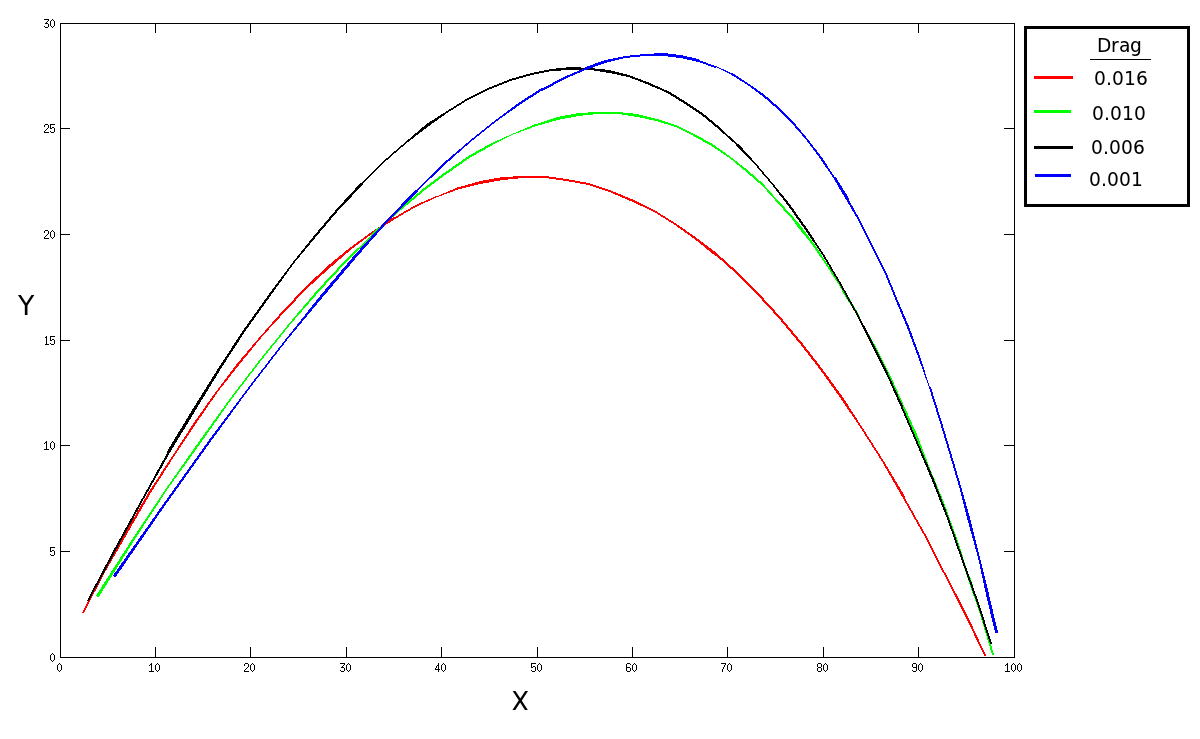
\includegraphics[width=3.5in]{fig2}
\caption{Figure shows different Trajectories used for training. These are obtained by varying the drag coefficient $C_{D}$}
\label{fig:fig2}
\end{figure}

\subsection{Data Representation and Retrieval}
The model is composed of the following processes:
\begin{itemize}
\item{
    \emph{Probabilistic data encoding:} The data is encoded in a two stage process. First, I determine the latent space of the trajectory motion by estimating the optimal Gaussian Mixture Model (GMM) to encode the motions. Second, we encode the dynamics of the motions (i.e. the transition across the states of the GMM), using Hidden Markov Model(HMM). This is the same approach as followed in \cite{ref:7}.
}    
\item{
    \emph{Optimal trajectory generation:} I compute the optimal trajectory for a new configuration via Gaussian Mixture Regression (GMR) and Lagrange optimizer if any constraints are placed.
}    
\end{itemize}

\subsubsection{Probabilistic data encoding}
To avoid making too many assumptions on the spatio-temporal variability of the dataset, I use a HMM with the most general architecture, such as a fully connected continuous HMM, with full covariance matrix, describing the output variables distribution. However, using such a model requires the estimation of a large set of parameters, which can be achieved only with a large dataset. However, to program efciently a robot by demonstration, the demonstrator should not have to perform more than a few (5 to 10) demonstrations. This means that the set of parameters to learn is quite large, compared to the amount of training data. 

The standard Expectation-Maximization (EM) algorithm used to estimate the HMM parameters starts from initial estimates, and converges to the nearest local maximum of the likelihood function. Thus, initialization highly affects the model performance. To better estimate the state distribution of the HMM, I perform first a rough clustering of the data using k-means. Next, I estimate a Gaussian Mixture Model (GMM) by EM, using the k-means clusters at initialization. Finally, the dynamics, i.e. transitions across states, are encoded in a HMM, with the GMM state variable distribution.

\begin{itemize}
\item[a)]{
    \textbf{Gaussian Mixture Model (GMM):} A dataset of N data of dimensionality D, X = \{$\vec{x(t_{1})}, \vec{x(t_{1})},\dots,\vec{x(t_{N})}$\} with $\vec{x(t_{n})} \in R^{D}$ is modelled by a multivariate Gaussian mixture of K-components
    \begin{equation}
        p(\vec{x(t_{n})}) = \sum_{k=1}^K \pi_{k} N (\vec{x(t_{n})}; \vec{\mu_{k}}, \Sigma_{k})
    \end{equation}
    where $\pi_{k}$ is the prior probability on the Gaussian component k, and $N (\vec{x(t_{n})}; \vec{\mu_{k}}, \Sigma_{k})$ is the D-Dimensional Gaussian density of component k. $\vec{\mu_{k}}$ and $\Sigma_{k}$ are the mean and covariance matrix of the multivariate Gaussian k. \{$\pi_{k}, \vec{\mu_{k}} , \Sigma_{k}$\} are estimated using the Expectation-Maximization (EM) algorithm.
}    
\\
\item[b)]{
    \textbf{Hidden Markov Model (HMM):} Similarly to Gaussian Mixture Models, Hidden Markov Models use a mixture of multivariate Gaussians to describe the distribution of the data.  The difference is that HMM also encapsulate the transitions probabilities between the Gaussians. It offers, thus, a way of describing probabilistically the temporal variations of the data.

    Let \{$\Pi$, A, B \} be, respectively, the initial state distribution, the transition probabilities between the states, and the multivariate output data distribution. In my experiments, I compute only \{$\Pi$, A\} by Baum-Welch algorithm, and set $B = {\vec{\mu_{k}}, \Sigma_{k}}_{k=1}^{K}$, which are the state distributions learned by the GMM. 
    
    In order to measure the similarity between a new trajectory and the ones encoded in the model, I run the forward-algorithm, an iterative procedure to estimate the likelihood that the observed data could have been generated by the model.
}
\\
\item[c)]{
    \textbf{Gaussian Mixture Regression (GMR):} To reconstruct the trajectory from the GMM/HMM encoding, after training and generalization over the demonstrations, I apply a Gaussian Mixture Regression (GMR). For a D-Dimensional variable $\vec{x} \in R^{D}$, the means and covariance matrices given by the GMM/HMM representation for component k are given by $\vec{\mu}_{kX}^{H}$ and ${\Sigma}_{kX}^{H}$. The regression is done along the time index. We compute the means and covariance matrices of the set of observations \{$t, \vec{x}(t)$\} with dimension (D+1). Note that the sole time-indexed covariances matrices and means are estimated, since the rest of the means and covariance matrices \{$\vec{\mu}_{kX}^{H}$, ${\Sigma}_{kX}^{H}$\} have already been estimated:
    \begin{equation}
        \vec{\mu}_{k}^{R} = \{\vec{\mu}_{kt}^{R}, \vec{\mu}_{kx_{1}}^{H}, \vec{\mu}_{kx_{2}}^{H}, \dots, \vec{\mu}_{kx_{D}}^{H}\}
    \end{equation}

    \begin{equation}
        {\Sigma}_{k}^{R} = \begin{pmatrix} {\Sigma}_{kt}^{R}&{\Sigma}_{ktX}^{R}\\ \\ {\Sigma}_{kXt}^{R}&{\Sigma}_{kX}^{H} \end{pmatrix}
    \end{equation}
    The Gaussian Mixture Regression estimates:
    \begin{equation}
        \vec{x}^{d}(t) = \sum_{k=1}^{K} \beta_{k}(t)\vec{x}_{k}^{d}(t)
    \end{equation}

    \begin{equation}
        \beta_{k}(t) = \frac{\pi_{k}N(t;\mu_{kt}^{R},\Sigma_{kt}^{R})}{\sum_{i=1}^{K}\pi_{i}N(t;\mu_{it}^{R},\Sigma_{it}^{R})}
    \end{equation}

    \begin{equation}
        \vec{x}_{k}^{d}(t) = \vec{\mu}_{kX} + {\Sigma}_{kXt}^{R} {{\Sigma}_{kt}^{R}}^{-1} (t - \mu_{kt})
    \end{equation}

    $\vec{x}_{k}^{d}(t)$ are the regression output for each associated Gaussian component k, $\beta_{k}(t)$ the corresponding weight, that measures the relative influence of component k, and $\pi_{k}$ the prior probability. $\vec{x}^{d}(t)$ is the desired trajectory, a generalized form of the motion learned during training. The time dependent inverse covariance of $\vec{x}(t)$ is estimated by:

    \begin{equation}
        W^{x}(t)= \begin{pmatrix}{\sum_{k=1}^{K} \beta_{k}(t) {\Sigma}_{k}^{R})}\end{pmatrix}^{-1}
    \end{equation}
}
\end{itemize}

Figure ~\ref{fig:fig3} shows the results of GMM encoding of the data and the generalized trajectory retrieved via GMR.

%% Figure3
\begin{figure}[!t]
\centering
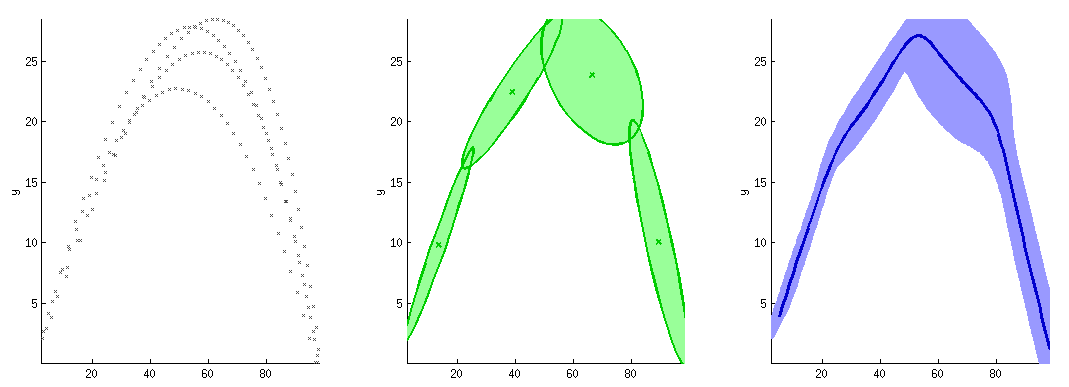
\includegraphics[width=3.5in]{fig3}
\caption{The first subfigure shows the different demonstration trajectories, the second subfigure shows the GMM encoding (no. of states =  4) of the trajectories and the third subfigure shows the retrieved generalized trajectory via GMR.}
\label{fig:fig3}
\end{figure}

\subsection{Continuous Learning and Data Storage}
In lifelong learning, the robot is expected to learn continuously over time and update its internal model to accurately reproduce trajectory. In doing so, there needs to be a bound on the memory when the no. of input trajectories explode. I have researched on this problem and using the proposed data representation and encoding, I show that the memory required to store such a model is substantially small when compared to storing each of the individual demonstrations. The following section explains my approach in detail. 

To demonstrate my method, I use the example of the projectile trajectories. In the normal case, one needs to store all the trajectories in order to efficiently represent the physics model. However, using the data representation approach detailed above, we only need to store the priors, means and covariance matrices of k components describing the demonstrations. 

In lifelong learning, if a new trajectory is required to be processed by the system, depending on how much variance we allow within a single class of trajectories, a decision needs to be made as to whether we include it in one of the existing trajectory classes or split it into a new class. There is a fundamental assumption of an already existing minimal model for this approach to work. Hence, the major advantage in my approach is that I store trajectory classes instead of the actual trajectories. Another advantage is instead of storing all the data points within a trajectory, I replace them with the GMM encoded priors, means and covariances matrices of the components describing the trajectory. The math equations of my method are described below.

Let,

\begin {itemize}
\item[]{\textit{K} = total no. of trajectories.}
\item[]{\textit{N} = total no. of trajectory splits.}
\item[]{\textit{n} = no. of states in the gaussian mixture model.}
\item[]{\textit{m} = no. of gaussian mixture components.}
\item[]{\textit{$\epsilon$} = threshold value of trajectory class variation.}
\item[]{\textit{$traj_{points}$} = no. of data points per trajectory.} 
\item[]{\textit{$\sigma$} = SD of the components in the trajectory class.} 
\item[]{\textit{$\mu$} = mean of the components in the trajectory class.} 
\item[]{\textit{$\sigma^\prime$} = SD of the components in the updated trajectory class.} 
\item[]{\textit{$\mu^\prime$} = mean of the components in updated trajectory class.} 
\item[]{\textit{$\Delta_{encode}$} = change of variation in updated trajectory class.} 
\item[]{\textit{$GMM_{encode}$} = variation of the trajectory class (0 - 1).} 
\item[]{\textit{$GMM_{memory}$} = used memory with GMM encoding.} 
\item[]{\textit{$Regular_{memory}$} = used memory without GMM.} 
\item[]{\textit{$bytes_{double}$} = no. of bytes to store a double value} 
\end {itemize}

Assume that there is an existing model, when a new trajectory is fed into the robot to process, a decision needs to be made whether the new trajectory can be put in one of the existing trajectory classes or a new split needs to be made. To make this decision, I compute the variation of all existing trajectory classes $\Delta_{encode}$ up on including the new trajectory as below,

% Delta_Encode equation
\begin{equation}
\Delta_{encode} = \frac{\sum_{i=1}^m \sum_{j=1}^n \sum_{k=1}^n |\sigma_{ijk} - \sigma_{ijk}^\prime| + \sum_{i=1}^m \sum_{j=1}^n |\mu_{ij} - \mu_{ij}^\prime|}{\epsilon}.
\end{equation}

The $GMM_{encode}$ is a scaled version of $\Delta_{encode}$ which varies between 0 to 1 and is computed as below,
% Conditional 
\[
    \text{$GMM_{encode}$}= 
\begin{cases}
    1, & \text{if $\Delta_{encode}$} \geq 1\\
    \text{$\Delta_{encode}$}, & \text{otherwise}
\end{cases}
\]

If the $GMM_{encode}$ value is more towards 0, it indicates that the trajectory class has little or no variation and hence can accomodate newer trajectories. As and when, the $GMM_{encode}$ nears 1, it indicates that a split is required as the variation limit has already been reached in the existing class.

The memory usage with and without GMM encoding can be computed as below,
% Memory Requirement
\begin{equation}
GMM_{memory} = N * bytes_{double} * ( nm + n^{2}m + n ).
\end{equation}
\begin{equation}
Regular_{memory} = K * bytes_{double} * m * traj_{points}.
\end{equation}

\section{Experimental Results}
For the experiments, I produced 100 demonstration trajectories using the Physics model outlined in Section IIA. Each of the trajectory has 50 data points and captures 3 components namely horizontal position \emph{x}, vertical position \emph{y} and the time \emph{t}. These trajectories are used to validate my method in the following sections.

\subsection{Splitting trajectory classes}
%% Figure4
\begin{figure}[!t]
\centering
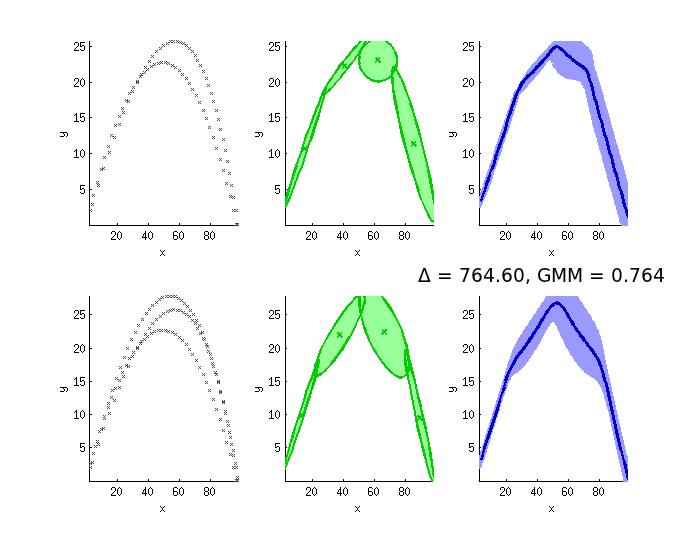
\includegraphics[width=3.5in]{fig4}
\caption{The figure shows the effect of including a new trajectory in an existing trajectory class. $\Delta_{encode} = 764.60, GMM_{encode} = 0.764, \epsilon=1000$}
\label{fig:fig4}
\end{figure}

%% Figure5
\begin{figure}[!t]
\centering
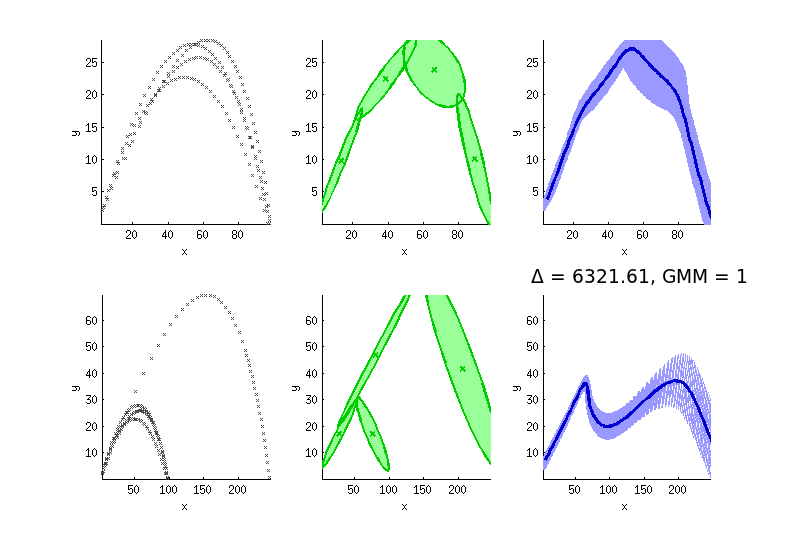
\includegraphics[width=3.5in]{fig5}
\caption{The figure shows the effect of including a new trajectory in an existing trajectory class. $\Delta_{encode} = 6321.61, GMM_{encode} = 1, \epsilon=1000$}
\label{fig:fig5}
\end{figure}

%% Figure6
\begin{figure}[!t]
\centering
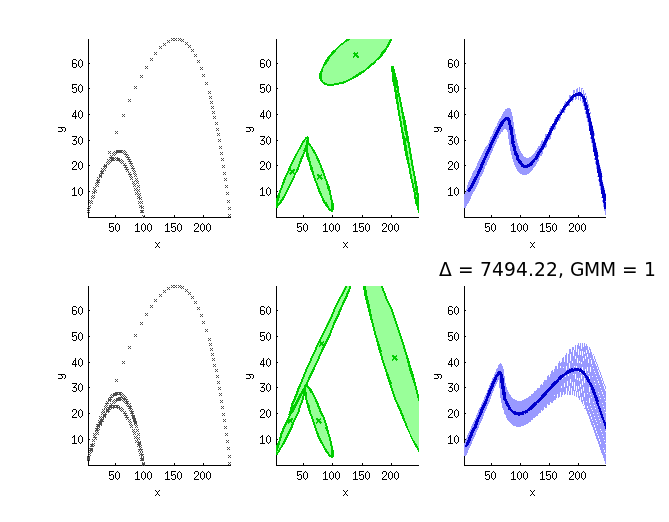
\includegraphics[width=3.5in]{fig6}
\caption{The figure shows the effect of including a new trajectory in an existing trajectory class. $\Delta_{encode} = 7494.22, GMM_{encode} = 1, \epsilon=1000$}
\label{fig:fig6}
\end{figure}

\begin{figure*}[!t]
\centerline{
    \subfigure[Case I]{
        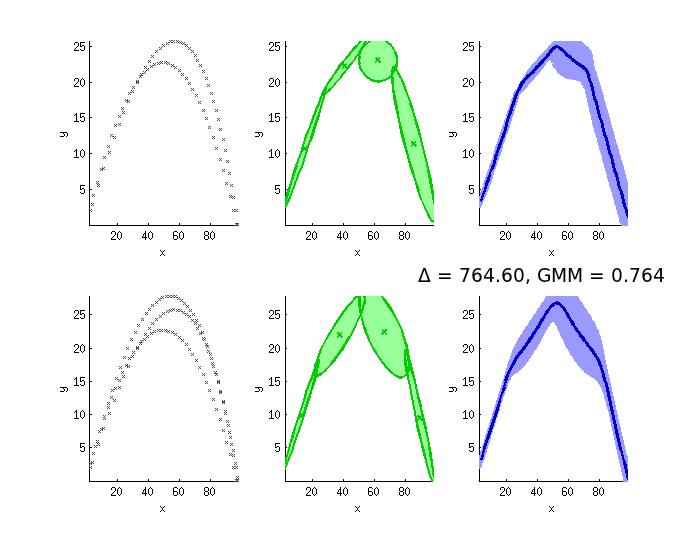
\includegraphics[width=3.5in]{fig4}
        \label{fig_4}
    }
    \subfigure[Case II]{
        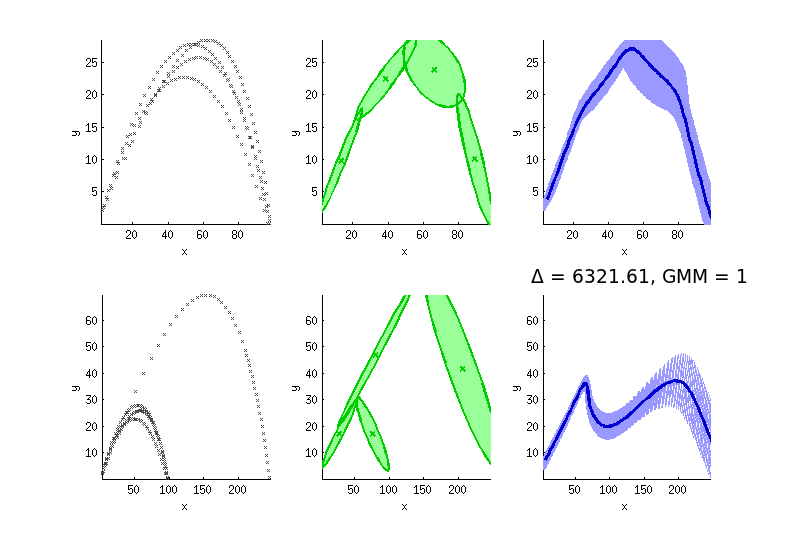
\includegraphics[width=3.5in]{fig5}
        \label{fig_second_case}
    }
}
\centerline{
    \subfigure[Case III]{
        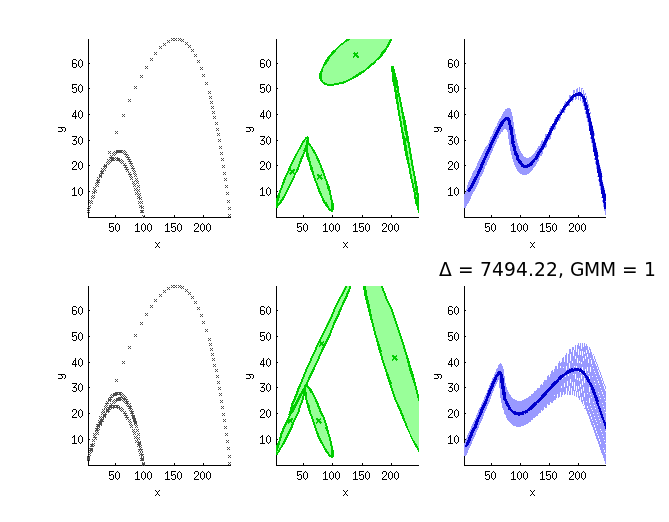
\includegraphics[width=3.5in]{fig6}
        \label{fig_second_case}
    }
}
\caption{Simulation results}
\label{fig_sim}
\end{figure*}



\section{Conclusion}
The conclusion goes here.

\section{Future Work}
Future work goes here.

% use section* for acknowledgement
\section*{Acknowledgment}


The authors would like to thank...

\begin{thebibliography}{1}

\bibitem{ref:1}
Vijaykumar Gullapalli,  Judy A. Franklin, and Hamid Benbrahim.  \emph{Acquiring robot skills via reinforcement  learning. IEEE Control Systems}, i72(  1708):  13-24, February  1994. 
\bibitem{ref:2}
Pattie Maes and Rodney A. Brooks.  \emph{Learning to coordinate behaviors.} In Proceedings Eighth National Conferenceon Artificial Intelligence,  pages 796-802, Cambridge, MA, 1990.  AAAI, The MIT Press. 
\bibitem{ref:3}
D.  A. Pomerleau.  \emph{ALVINN: an  autonomous land vehicle  in  a neural network.}  Technical Report CMU-CS-89- 107, Computer Science Dept. Camegie Mellon University, Pittsburgh PA, 1989.
\bibitem{ref:4}
Tom M. Mitchell.  \emph{Becoming  increasingly reactive.}  In Proceedings of1990 AAAl Conference, Menlo Park, CA, August  1990.  AAAI, AAAl Press I The MIT Press. 
\bibitem{ref:5}
Sebastian B. Thrun and Tom M. Mitchell.  \emph{Lifelong robot learning. Robotics and Autonomous Systems, 1993.} Also appeared as Technical Report IAI-TR-93-7.  University of Bonn, Dept.  of Computer Science 111.
\bibitem{ref:6}
Thrun, S. B. 1994. \emph{A Lifelong Learning Perspective for Mobile Robot Control.} In Proceedings of the IEEE/RSJ/GI International Conference on Intelligent Robots and Systems, 23-30. Washington, D.C.: IEEE Computer Society.
\bibitem{ref:7}
Calinon S, Guenter F, Billard A (2006). \emph{On Learning the Statistical Representation of a Task and Generalizing it to Various Contexts.}  Proc IEEE/ICRA 2006.

\end{thebibliography}

% that's all folks
\end{document}
